\documentclass[border=10pt]{standalone}

\usepackage{tikz}
\usepackage{tikzsymbols}
\usetikzlibrary{calc,patterns,shapes.geometric}

\def\centerarc[#1](#2)(#3:#4:#5){\draw[#1] ($(#2)+({#5*cos(#3)},{#5*sin(#3)})$) arc (#3:#4:#5);}

\begin{document}
	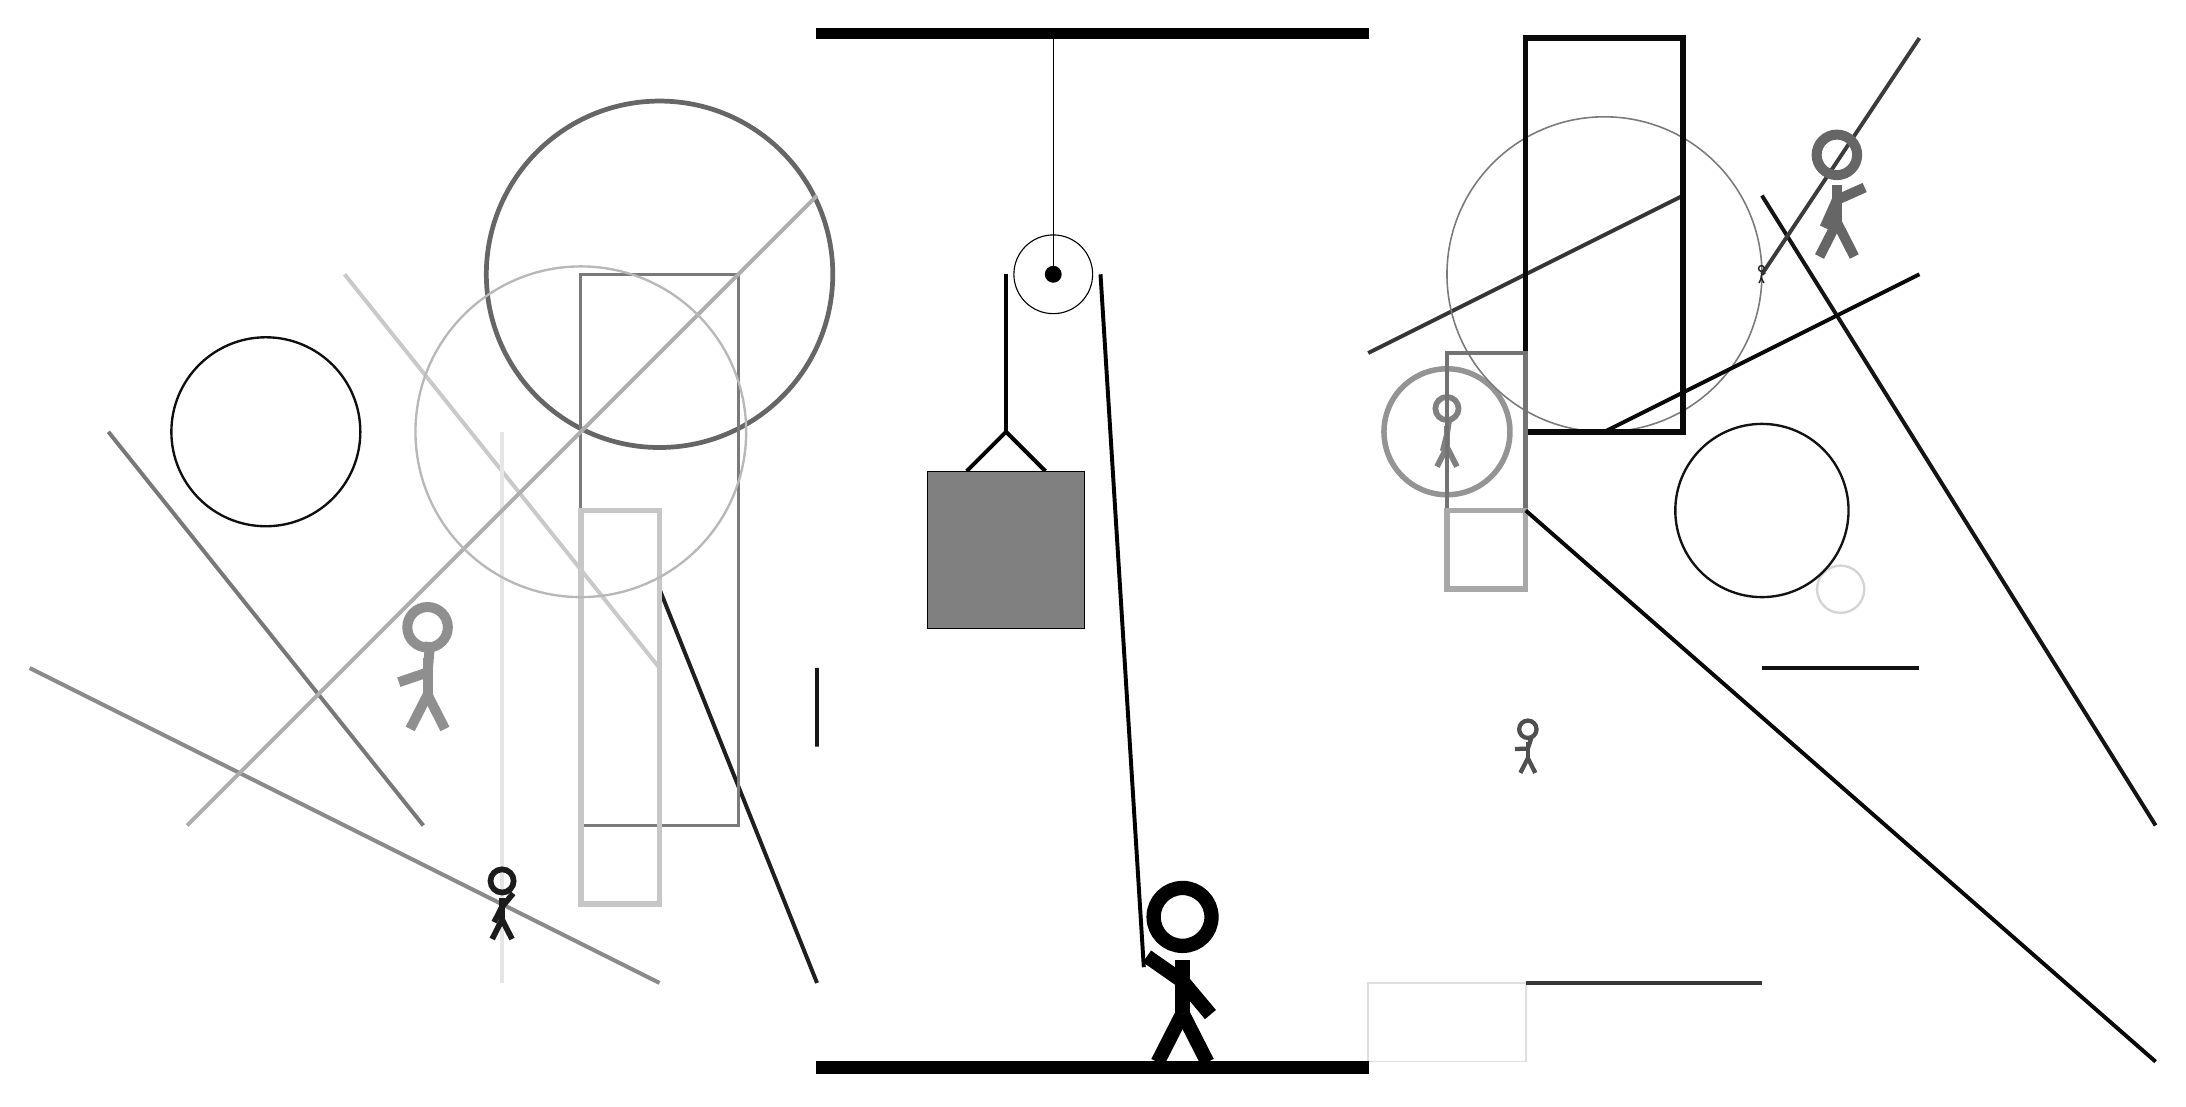
\begin{tikzpicture}
		%%%%% START %%%%%
		
		\draw[fill=black] (-2, 10) rectangle (5, 10.125);
		
		\draw (1, 7) circle (0.5);
		\draw[fill=black] (1, 7) circle (0.1);
		\draw (1, 10) -- (1, 7);
		
		\draw[line width=0.5mm] (-0.1, 4.5) -- (0.4, 5.0) -- (0.9, 4.5);
		\draw[fill=black!50] (-0.6, 4.5) rectangle (1.4, 2.5);
		
		\draw [line width=0.7mm, color=black!42](6, 5) circle (0.8);
		
		\draw[line width=0.5mm, color=black!79](5, 6) -- (9, 8);
		\draw [line width=0.2mm, color=black!52](8, 7) circle (2.0);
		\node[line width=0.3mm, color=black!44] at (-7, 2) {\Strichmaxerl[7][19][85]};
		\draw[line width=0.7mm, color=black!96] (7, 10) rectangle (9, 5);
		
		\node[line width=0.4mm, color=black!50] at (6, 5) {\Strichmaxerl[4][76][81]};
		
		\node[line width=0.6mm, color=black!69] at (7, 1) {\Strichmaxerl[3][2][72]};
		\draw [line width=0.6mm, color=black!60](-4, 7) circle (2.2);
		\draw[line width=0.5mm, color=black!92](10, 8) -- (15, 0);
		\draw[line width=0.5mm, color=black!21](-4, 2) -- (-8, 7);
		\draw[line width=0.5mm, color=black!88](-2, -2) -- (-4, 3);
		\draw[line width=0.5mm, color=black!96](8, 5) -- (12, 7);
		\draw[line width=0.5mm, color=black!77](10, 7) -- (12, 10);
		
		\draw[line width=0.6mm, color=black!55] (6, 3) rectangle (7, 6);
		\draw[line width=0.2mm, color=black!13] (5, -2) rectangle (7, -3);
		\draw[line width=0.5mm, color=black!79](10, -2) -- (7, -2);
		
		\draw [line width=0.3mm, color=black!17](11, 3) circle (0.3);
		\draw[line width=0.4mm, color=black!52] (-3, 7) rectangle (-5, 0);
		\draw [line width=0.3mm, color=black!93](10, 4) circle (1.1);
		
		\draw[line width=0.5mm, color=black!53](-7, 0) -- (-11, 5);
		\draw [line width=0.3mm, color=black!94](-9, 5) circle (1.2);
		
		\draw[line width=0.6mm, color=black!91] (-2, 1) rectangle (-2, 2);
		
		\draw[line width=0.5mm, color=black!46](-4, -2) -- (-12, 2);
		\draw[line width=0.7mm, color=black!22] (-4, -1) rectangle (-5, 4);
		\draw[line width=0.5mm, color=black!93](10, 2) -- (12, 2);
		
		\draw[line width=0.7mm, color=black!34] (6, 3) rectangle (7, 4);
		
		\node[line width=0.5mm, color=black!60] at (11, 8) {\Strichmaxerl[7][66][24]};
		\draw[line width=0.2mm, color=black!47] (7, 9) rectangle (7, 9);
		
		\node[line width=0.2mm, color=black!85] at (10, 7) {\Strichmaxerl[1][82][27]};
		\draw[line width=0.5mm, color=black!10](-6, 5) -- (-6, -2);
		\draw[line width=0.5mm, color=black!97](7, 4) -- (15, -3);
		
		\node[line width=0.5mm, color=black!89] at (-6, -1) {\Strichmaxerl[4][63][50]};
		\draw[line width=0.5mm, color=black!32](-2, 8) -- (-10, 0);
		
		\draw [line width=0.3mm, color=black!28](-5, 5) circle (2.1);
		
		
		\draw[line width=0.5mm] (0.4, 7) -- (0.4, 5.0);
		\centerarc[line width=0.5mm](1, 7)(0:180:0.6);
		\draw[line width=0.5mm](1.6, 7) -- (2.15, -1.8);
		
		\node at (2.6, -1.9) {\Strichmaxerl[10][-35][-50]};
		
		\draw[fill=black] (-2, -3) rectangle (5, -3.15);
		
		%%%%% END %%%%%
	\end{tikzpicture}
\end{document}